%\documentclass[10pt]{article}
%\usepackage[utf8]{inputenc}
%\usepackage[T1]{fontenc}
%\usepackage{amsfonts}
%\usepackage{amssymb}
%\usepackage{geometry}
%\usepackage{pstricks,pst-eucl}
%\usepackage{tikz}
%\usepackage{graphics}
%\usepackage{pslatex}
%\usepackage{lscape}
%\usepackage{eurosym}
%\usepackage{skak}
%\usepackage{chessboard}

\documentclass[12pt, a4paper]{report}
%\documentclass[11pt, a4paper]{article}

%====================== PACKAGES ======================

\usepackage[french]{babel}
\frenchbsetup{StandardLists=true}
\usepackage{enumitem}
\usepackage{pifont}
\usepackage[utf8x]{inputenc}
\usepackage[T1]{fontenc}
%pour gérer les positionnement d'images
\usepackage{float}
\usepackage{amsmath}
\DeclareMathOperator{\dt}{dt}
\usepackage{graphicx}
\usepackage{tabularx}
\usepackage[colorinlistoftodos]{todonotes}
\usepackage{url}
%pour les informations sur un document compilé en PDF et les liens externes / internes
\usepackage[pdfborder=0]{hyperref}
\hypersetup{
	colorlinks = true
	}
%pour la mise en page des tableaux
\usepackage{array}
\usepackage{tabularx}
\usepackage{multirow}
\usepackage{multicol}
\setlength{\columnsep}{50pt}
%espacement entre les lignes
\usepackage{setspace}
%modifier la mise en page de l'abstract
\usepackage{abstract}
%police et mise en page (marges) du document
\usepackage[T1]{fontenc}
\usepackage[top=2cm, bottom=2cm, left=2cm, right=2cm]{geometry}
%Pour les galerie d'images
\usepackage{subfig}

\usepackage{pdfpages}
%\usepackage{tikz}

\usepackage{appendix}

\usepackage{comment}

\usepackage{skak}
\usepackage{chessboard}

%\usetikzlibrary{angles, quotes}
%\usetikzlibrary{decorations.pathmorphing}
%====================== INFORMATION ET REGLES ======================

%rajouter les numérotation pour les \paragraphe et \subparagraphe
\setcounter{secnumdepth}{4}
\setcounter{tocdepth}{4}

\hypersetup{							% Information sur le document
pdfauthor = {Stephan Runigo},			% Auteurs
pdftitle = {Recueil d'echec},			% Titre du document
pdfsubject = {Répertoire d'ouverture et parties},		% Sujet
pdfkeywords = {échec, ouverture},	% Mots-clefs
pdfstartview={FitH}}	% ajuste la page à la largeur de l'écran
%pdfcreator = {MikTeX},% Logiciel qui a crée le document
%pdfproducer = {} % Société avec produit le logiciel
%======================== DEBUT DU DOCUMENT ========================
%
\begin{document}
%
%régler l'espacement entre les lignes
\newcommand{\HRule}{\rule{\linewidth}{0.5mm}}
%
%présentation	%
%
%
\begin{titlepage}
%
~\\[1cm]

\begin{center}
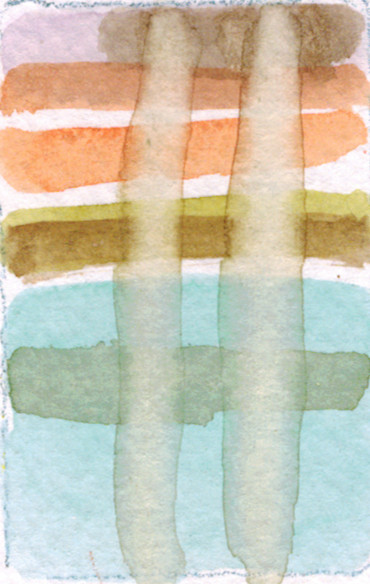
\includegraphics[scale=2]{./presentation/champ06}
\end{center}

\textsc{\Large }\\[0.5cm]

% Title \\[0.4cm]
\HRule

\begin{center}
{\huge \bfseries  Principes élémentaires\\
du jeu d'échec\\[0.4cm] }
\end{center}

\HRule \\[1.5cm]

\begin{center}
%\includegraphics[scale=0.3]{./presentation/ptoleme}
\end{center}

\begin{center}
%\includegraphics[scale=0.3]{./presentation/diagrammesInteractions}
\end{center}


% Author and supervisor
\begin{minipage}{0.4\textwidth}
\begin{flushleft} \large
\emph{Auteur:}\\
Stephan \textsc{Runigo}
\end{flushleft}
\end{minipage}
\begin{minipage}{0.4\textwidth}
\begin{flushright} \large
\emph{Illustration:}\\
Krikri
\end{flushright}
\end{minipage}

\vfill

% Bottom of the page
{\large \today}

\end{titlepage}

\newpage
\begin{center}
\Large
Résumé
\normalsize
\end{center}
\vspace{3cm}
\begin{itemize}[leftmargin=1cm, label=\ding{32}, itemsep=21pt]
\item {\bf Objet : Les ouvertures} .
\item {\bf Contenu : Principes élémentaires} .
\item {\bf Public concerné : Débutant} .
\end{itemize}

\vspace{3cm}



\vspace{3cm}


%

%
%\newpage
%~
%ne pas numéroter cette page
%\thispagestyle{empty}
	%\newpage

\tableofcontents
\thispagestyle{empty}
\setcounter{page}{0}
%ne pas numéroter le sommaire
%
%\newpage
%
%espacement entre les lignes d'un tableau
\renewcommand{\arraystretch}{1.5}
%
%====================== INCLUSION DES PARTIES ======================
%
~
\thispagestyle{empty}
%recommencer la numérotation des pages à "1"
\setcounter{page}{0}
\newpage
%	%
%
%
\newpage
%
\chapter{Principes stratégiques}

%Ce chapitre recense les principes stratégiques.

%%%%%%%%%%%%%%%%%%%%%%%%%%%%%%%%%%
\section{Ouverture}
%%%%%%%%%%%%%%%%%%%%%%%%%%%%%%%%%%

\begin{itemize}[leftmargin=2.7cm, label=\ding{32}, itemsep=0pt]%\end{itemize}
\item  {\bf Se dévelloper}
\item  {\bf Controler le centre}
\item  {\bf Roquer}
\end{itemize}

\begin{itemize}[leftmargin=2.7cm, label=\ding{32}, itemsep=0pt]%\end{itemize}
\item  {\bf Gagner des  temps de développement}
\item  {\bf Faire jouer ses pièces ensemble / les protéger}
\end{itemize}

%%%%%%%%%%%%%%%%%%%%%%%%%%
\section{Milieu de partie}
%%%%%%%%%%%%%%%%%%%%%%%%%%
\begin{itemize}[leftmargin=2.7cm, label=\ding{32}, itemsep=0pt]%\end{itemize}
\item  {\bf Repérer les faiblesses}
\item  {\bf Reconnaître les schémas tactiques}
\item  {\bf Considérer les échanges de même valeur}
\item  {\bf Évaluer les finales}
\end{itemize}

Mettre une tour sur la 7$^\text{ème}$ rangée dès que cela est possible.
Doubler les tours sur la 7$^\text{ème}$ rangée dès que cela est possible.

%%%%%%%%%%%%%%%%%%%%%%%%%%%%%%%%%%
\section{Exemple de plan}
%%%%%%%%%%%%%%%%%%%%%%%%%%%%%%%%%%

\begin{itemize}[leftmargin=2.7cm, label=\ding{32}, itemsep=0pt]%\end{itemize}
\item  {\bf Pièges à l'ouverture}
\item  {\bf Attaque de mat}
\item  {\bf Attaque d'une faiblesse}
\end{itemize}

\begin{itemize}[leftmargin=2.7cm, label=\ding{32}, itemsep=0pt]%\end{itemize}
\item  {\bf Défense} : contrer le plan adverse
\item  {\bf Consolidation}
\end{itemize}

%%%%%%%%%%%%%%%%%%%%%%%%%%%%%%%%%%
%\subsection{Finale}
%%%%%%%%%%%%%%%%%%%%%%%%%%%%%%%%%%


%%%%%%%%%%%%%%%%%%%%%%%%%%%%%%%%%%%%%%%%%%%%%%%%%%%%%%%%%%%%%%%%%%%%%%%%

%

%\input{./utilisation/exemple.tex}

\section{Milieu de partie}
%
%
Au cours du milieux de partie,

\begin{itemize}[leftmargin=2.7cm, label=\ding{32}, itemsep=0pt]%\end{itemize}
\item  {\bf Repérer les faiblesses}
\item  {\bf Reconnaître les schémas tactiques}
\item  {\bf Considérer les échanges de même valeur}
\item  {\bf Évaluer les finales}
\end{itemize}

Mettre une tour sur la 7$^\text{ème}$ rangée dès que cela est possible.
Doubler les tours sur la 7$^\text{ème}$ rangée dès que cela est possible.

%%%%%%%%%%%%%%%%%%%%%
\subsection{Élaboration d'un plan}
%%%%%%%%%%%%%%%%%%%%%

Il est important de jouer des coups qui on du {\it sens}. Pour cela, il doivent suivre un plan, par exemple : 

\begin{itemize}[leftmargin=2.7cm, label=\ding{32}, itemsep=0pt]%\end{itemize}
\item  {\bf Pièges à l'ouverture}
\item  {\bf Attaque de mat}
\item  {\bf Attaque d'une faiblesse}
\item  {\bf Défense, consolidation}
\end{itemize}

%%%%%%%%%%%%%%%%%%%%%
%\subsection{Repérer les faiblesses}
%%%%%%%%%%%%%%%%%%%%%
%
%%%%%%%%%%%%%%%%%%%%%
%\subsection{Reconnaître les schémas tactiques}
%%%%%%%%%%%%%%%%%%%%%
%
%%%%%%%%%%%%%%%%%%%%%
%\subsection{Considérer les échanges de même valeur}
%%%%%%%%%%%%%%%%%%%%%
%
%%%%%%%%%%%%%%%%%%%%%
%\subsection{Évaluer les finales}
%%%%%%%%%%%%%%%%%%%%%

%%%%%%%%%%%%%%%%%%%%%%%%%%%%%%%%%%%%%%%%%%%%%%%%%%%%%%%%%%%%%%%%%%%%%%%%


%%%%%%%%%%%%%%%%%%%%%%%%%%%%%%%%%%%%%%%%%%%%%%%%%%%%%%%%%%%%%%%%%%%%%%%%

%

%\input{./utilisation/exemple.tex}

\section{Finale}


On met la tour derrière le pion passé

%

%\input{./utilisation/exemple.tex}

\section{Fous et jeu de couleur}
%
Les pièces mineures valent environ 3 pions.
L'ouverture conduit généralement à des positions où des échanges de pièces mineures sont possible.
Ces échanges sont parfois avantageux.

%%%%%%%%%%%%%%%%%%%%%
\subsection{Bon fou / mauvais fou}
%%%%%%%%%%%%%%%%%%%%%
%
Lorsque la structure des pions centraux est fixé et qu'il sont sur une certaine couleur, notre bon fou est celui de couleur opposé. En effet, nos pions ne lui enlève pas d'espace. L'autre fou est notre mauvais fou car nos propre pions centraux lui enlève de l'espace.
\subsubsection{fou actif/ fou passif}
Si le mauvais fou est devant sa structure de pion, il est actif, il tape dans le camp adverse, il peut être plus fort que le bon fou.
%%%%%%%%%%%%%%%%%%%%%
\subsection{fous de couleur opposée}
%%%%%%%%%%%%%%%%%%%%%
Après des échanges chaque joueur ne possède plus qu'un fous, et  que ces deux fous sont de couleur opposé.

Alors,

\begin{itemize}[leftmargin=1.7cm, label=\ding{32}, itemsep=0pt]%\end{itemize}
\item  {\bf placer ses pions sur la couleur du fous adverse} : enlève de l'espace au fou adverse, donne de l'espace à notre fou, très bon stratégiquement si nos pions sont difficilement attacable ou facilement défendable.
\item  {\bf placer ses pions sur la couleurs de notre fous} : nos pions ne peuvent plus être attaquer par le fou adverse, bon stratégiquement si nos pions étaient facilement attacable, difficilement défendable et si notre fou est actif.
\end{itemize}




%%%%%%%%%%%%%%%%%%%%%
\subsection{Paire de fous}
%%%%%%%%%%%%%%%%%%%%%
%%%%%%%%%%%%%%%%%%%%%
\subsubsection{Qui possède les fous possède l'avenir}
%%%%%%%%%%%%%%%%%%%%%
Lorsqu'on envisage l'échange de pièces mineurs, conserver la paire de fou procure généralement un avantage stratégique à long terme. En début de partie ou lorsque la position est fermée, un cavalier est plus fort qu'un fou. Lorsque la position est ouverte et en fin de partie, un fou est plus fort qu'un cavalier. 
%
%%%%%%%%%%%%%%%%%%%%%%%%%%%%%%%%%%%%%%%%%%%%%%%%%%%%%%%%%%%%%%%%%%%%%%%%
%Parties d-échecs pédagogiques avec progression 🎓 1300 elo.mp4
% Capture du 2022-03-13 21-18-02.png : 35 minute
%  Protéger avec le fou permet de se débarasser du problème de son développement

%Parties d-échecs pédagogiques avec progression 🎓 1300 elo.mp4
%Capture du 2022-03-13 22-04-16.png : 1 h 11 min
%  Les pions adverses sont sur case blanche, l'adversaire est donc faible sur case noir, échanger le fou de case blanche contre un cavalier va donner un avantage matériel sur les cases noires.

%Capture du 2022-03-13 22-21-45.png, 1 h 20 min
% Pour augmenter l'avantage sur les cases noires, Te5?!


%PSG-ed.mp4, 16 min
%Capture du 2022-03-13 23-05-03.png
%finale égale 
%%%%%%%%%%%%%%%%%%%%%%%%%%%%%%%%%%%%%%%%%%%%%%%%%%%%%%%%%%%%%%%%%%%%%%%

%%%%%%%%%%%%%%%%%%%%%%%%%
\section{Roques opposés}
%%%%%%%%%%%%%%%%%%%%%%%
%
%\subsection{Prendre le centre}

%


%%%%%%%%%%%%%%%%%%%%%%%%%%%%
\section{Roques symétriques}
%%%%%%%%%%%%%%%%%%%%%%%%%%%%


%%%%%%%%%%%%%%%%%%%%%%%%%%%%%%%%%%%%%%%%%%%%%%%%%%%%%%%%%%%%%%%%%%%%%%%%



%\newpage
%
%\chapter{Principes tactiques}

%Ce chapitre traite des principes tactiques.

%
\section{Ouvertures}
%
Stratégiquement, l'ouverture consiste à

\begin{itemize}[leftmargin=2.7cm, label=\ding{32}, itemsep=0pt]%\end{itemize}
\item  {\bf Se dévelloper}
\item  {\bf Controler le centre}
\item  {\bf Roquer}
\end{itemize}

Au cours de l'ouverture, il est souvent interessant de
\begin{itemize}[leftmargin=2.7cm, label=\ding{32}, itemsep=0pt]%\end{itemize}
\item  {\bf Gagner des  temps de développement}
\item  {\bf Faire jouer ses pièces ensemble / les protéger}
\end{itemize}

%%%%%%%%%%%%%%%%%%%%%
\subsection{Prendre le centre}
%%%%%%%%%%%%%%%%%%%%%
%
L'occupation du centre consiste à placer une pièce au centre. Cela peut être un pion ou une pièce mineure. Contrôler le centre consiste à placer une pièce qui attaque une ou plusieurs case du centre.


%%%%%%%%%%%%%%%%%%%%%
\subsection{Se développer}
%%%%%%%%%%%%%%%%%%%%%
%
Le développement consiste à sortir ses pièces mineures. Il faut éviter de jouer deux fois la même pièce dans cette phase.

%Parties d-échecs pédagogiques avec progression 🎓 1300 elo.mp4 : {\it Cf3 d4 d5 Cf6 Ce5}

%%%%%%%%%%%%%%%%%%%%%
\subsection{Roquer}
%%%%%%%%%%%%%%%%%%%%%
%
Le roque permet de mettre le roi à l'abri mais également de mettre les tours en liaison. C'est lorsque les tours sont en liaison que l'ouverture est terminé.


%%%%%%%%%%%%%%%%%%%%%
\subsection{Gagner des  temps de développement}
%%%%%%%%%%%%%%%%%%%%%
Créer une menace en se développant oblige l'adversaire à contrer cette menace, et permet de gagner du temps. Obliger l'adversaire à jouer deux fois la même pièce permet de retarder son développement.

Avancer un pion centrale pour attaqer un cavalier est souvent un bon coup.

%%%%%%%%%%%%%%%%%%%%%
\subsection{Faire jouer ses pièces ensemble}
%%%%%%%%%%%%%%%%%%%%%

Les pièces doivent se protéger entre elles et attaquer une même case faible de l'adversaire.

%%%%%%%%%%%%%%%%%%%%%%%%%%%%%%%%%%%%%%%%%%%%%%%%%%%%%%%%%%%%%%%%%%%%%%%%


%%%%%%%%%%%%%%%%%%%%%%%%%%%%%%%%%%%%%%%%%%%%%%%%%%%%%%%%%%%%%%%%%%%%%%%%

%
%%%%%%%%%%%%%%%%%%%%%
\section{Découverte}
%%%%%%%%%%%%%%%%%%%%%

Une attaque à la découverte est l'attaque d'une pièce par une pièce. En général, ces attaques conduisent à prendre un avantage.

%%%%%%%%%%%%%%%%%%%%%%%%%%%%%%%%%%%%%%%%%%%%%%%%%%%%%%%%%%

%
%%%%%%%%%%%%%%%%%%%%%
\section{Fourchette}
%%%%%%%%%%%%%%%%%%%%%

Une attaque double (ou fourchette) est l'attaque de deux pièces par une pièce. En général, ces attaques conduisent à prendre un avantage.

%%%%%%%%%%%%%%%%%%%%%%%%%%%%%%%%%%%%%%%%%%%%%%%%%%%%%%%%%%

%

%
%%
%
\newpage
%
\chapter{Ouvertures}

Ce chapitre traite des ouvertures.



%\input{./utilisation/exemple.tex}

\section{Principes élémentaires}
%
%%%%%%%%%%%%%%%%%%%%%
\subsection{Prendre le centre}
%%%%%%%%%%%%%%%%%%%%%
%
L'occupation du centre consiste à placer une pièce au centre. Cela peut être un pion ou une pièce mineure. Contrôler le centre consiste à placer une pièce qui attaque une ou plusieurs case du centre.

\begin{center}
\newgame
\mainline{1. e4 }
\def\empharea{ e4-e4 }
\chessboard[color=red,
	markstyle=color,markfields=d5,
	emphstyle=\color{green},
	empharea=\empharea]
\end{center}

Le pion e4 occupe une case centrale et contrôle la case centrale (d5). C'est un bon coup.

\begin{center}
\newgame
\mainline{1. Nf3 }
\def\empharea{ f3-f3 }
\chessboard[color=red,
	markstyle=color,markfields=d4,
	markstyle=color,markfields=e5,
	emphstyle=\color{green},
	empharea=\empharea]
\end{center}

Le cavalier f3 contrôle les deux cases centrales d4 et e5.

\newgame

\mainline{1. e4 e5 2. Nf3 Nc6}

\begin{center}
\chessboard
\end{center}

%\newchessgame
\newgame

\def\empharea{ h8-f4 }
\chessboard[emphstyle=\color{red},
empharea=\empharea]



%%%%%%%%%%%%%%%%%%%%%
\subsection{Se développer}
%%%%%%%%%%%%%%%%%%%%%
%

\subsubsection{Sortir les pièces mineures}


\subsubsection{Gagner du temps}

Créer une menace en se développant oblige l'adversaire à contrer cette menace. 



%%%%%%%%%%%%%%%%%%%%%
\subsection{Roquer}
%%%%%%%%%%%%%%%%%%%%%
%

%%%%%%%%%%%%%%%%%%%%%%%%%%%%%%%%%%%%%%%%%%%%%%%%%%%%%%%%%%%%%%%%%%%%%%%%


%%%%%%%%%%%%%%%%%%%%%%%%%%%%%%%%%%%%%%%%%%%%%%%%%%%%%%%%%%%%%%%%%%%%%%%%

%%%%%%%%%%%%%%%%%%%%%%%%%%%%%%%%%%%%%%%%%%%%%%%%%%%%%%%%%%
%
\section{Jouer l'écossaise}
%
%%%%%%%%%%%%%%%%%%%%%%%%%%%%%%%%%%%%%%%%%%%%%%%%%%%%%%%%%%
%
%L'écossaise se caractérise par le coup \texttt{3. d4} après les coups classiques \texttt{1. e4 e5 2. Cf3 Cc6} :
Après les coups classiques, fréquement joués
\newgame

\mainline{1. e4 e5 2. Nf3 Nc6}

\begin{center}
\chessboard
\end{center}


L'écossaise se caractérise par le coup
%les blancs rentre généralement dans la partie espagnole ou la partie italienne. Il peuvent également rentré dans la partie écossaise
%\textit{Projet Cavalier e5, Tour e1}
\mainline{3. d4}

%\textit{Fréquent : }\textit{}
%\variation{4. e5}


%\mainline{4... Bg4}

\begin{center}
\chessboard
\end{center}












\newgame

\mainline{1. e4 e6 2. d4 d5 3. e5}

\begin{center}
\chessboard
\end{center}


\newgame

\textit{Projet Cavalier e5, Tour e1}
\mainline{1. e4 e6 2. d4 d5 3. pxd5}

\begin{center}
\chessboard
\end{center}


\newgame
%rnbqkbnr/pppppppp/8/8/8/8/PPPPPPPP/RNBQKBNR

\begin{center}
\chessboard{rnbqkbnr/pppppppp/8/8/8/8/PPPPPPPP/RNBQKBNR w KQkq - 0 1}
\end{center}



%\mainline{3. exd}
%%%%%%%%%%%%%%%%%%%%%%%%%%%%%%%%%%%%%%%%%%%%%%%%%%%%%%%%%

%%%%%%%%%%%%%%%%%%%%%%%%%%%%%%%%%%%%%%%%%%%%%%%%%%%%%%%%%%
%
\section{Jouer contre la Française}
%
%%%%%%%%%%%%%%%%%%%%%%%%%%%%%%%%%%%%%%%%%%%%%%%%%%%%%%%%%%
%
\newgame

\mainline{1. e4 e6 2. d4 d5}

\begin{center}
\chessboard
\end{center}

\textit{Projet Cavalier e5, Tour e1}
\mainline{3. pexd5 pexd5}

\textit{Fréquent : }
%\variation{4. e5}


%\mainline{4... Bg4}

\begin{center}
\chessboard
\end{center}

\newgame

\mainline{1. e4 e6 2. d4 d5 3. e5}

\begin{center}
\chessboard
\end{center}


\newgame

\textit{Projet Cavalier e5, Tour e1}
\mainline{1. e4 e6 2. d4 d5 3. pxd5}

\begin{center}
\chessboard
\end{center}


\newgame
%rnbqkbnr/pppppppp/8/8/8/8/PPPPPPPP/RNBQKBNR

\begin{center}
\chessboard{rnbqkbnr/pppppppp/8/8/8/8/PPPPPPPP/RNBQKBNR w KQkq - 0 1}
\end{center}



%\mainline{3. exd}
%%%%%%%%%%%%%%%%%%%%%%%%%%%%%%%%%%%%%%%%%%%%%%%%%%%%%%%%%

%%%%%%%%%%%%%%%%%%%%%%%%%%%%%%%%%%%%%%%%%%%%%%%%%%%%%%%%%%%
%
\section{Les ouvertures de MVL}
%
%%%%%%%%%%%%%%%%%%%%%%%%%%%%%%%%%%%%%%%%%%%%%%%%%%%%%%%%%%
%
%
% D'après la vidéo
%  MVL contre Nepo - le match des marlous.mp4
%
\newgame

\subsection{Réfutation de 1. g3}

\mainline{1. g3 h5 2. Bg2 h4}

\begin{center}
\chessboard
\end{center}

\mainline{3. d4 d5 4. c4 e6}

\mainline{5. Nc3 c6 }
 %\mainline{6. e4 dc4}

%\textit{Fréquent : }
%\variation{4. e5}

\begin{center}
\chessboard
\end{center}

%rnbqkbnr/pppppppp/8/8/8/8/PPPPPPPP/RNBQKBNR

\begin{center}
%\chessboard{rnbqkbnr/pppppppp/8/8/8/8/PPPPPPPP/RNBQKBNR w KQkq - 0 1}
\end{center}



%\mainline{3. exd}
%%%%%%%%%%%%%%%%%%%%%%%%%%%%%%%%%%%%%%%%%%%%%%%%%%%%%%%%%

%\input{./ouverture/.tex}

%

%
%\chapter{Milieu de partie}
%

%%%%%%%%%%%%%%%%%%%%%
\section{Faiblesses}
%%%%%%%%%%%%%%%%%%%%%

Détecter des faiblesses chez l'adversaire donne un plan (attaquer ces faiblesses). Détecter des faiblesses dans son propre camp permet de consolider sa position.


\subsection{Pion isolé}


\subsection{Pion arriéré}


\subsection{Pion avancé}

%%%%%%%%%%%%%%%%%%%%%%%%%%%%%%%%%%%%%%%%%%%%%%%%%%%%%%%%%%%%%%%%%%%%%%%%%%%

%

%%%%%%%%%%%%%%%%%%%%%
\section{Organisation des pièces}
%%%%%%%%%%%%%%%%%%%%%

\subsection{Consolidation}

\section{Protection}

\section{Attaque}

%%%%%%%%%%%%%%%%%%%%%%%%%%%%%%%%%%%%%%%%%%%%%%%%%%%%%%%%%%%%%%%%%%%%%%%%%%%

%

%%%%%%%%%%%%%%%%%%%%%
\section{Fourchette}
%%%%%%%%%%%%%%%%%%%%%

Une attaque double (ou fourchette) est l'attaque de deux pièces par une pièce. En général, ces attaques conduisent à prendre un avantage.

%%%%%%%%%%%%%%%%%%%%%%%%%%%%%%%%%%%%%%%%%%%%%%%%%%%%%%%%%%

%

%%%%%%%%%%%%%%%%%%%%%
\section{Découverte}
%%%%%%%%%%%%%%%%%%%%%

Une attaque à la découverte est l'attaque d'une pièce par une pièce. En général, ces attaques conduisent à prendre un avantage.

%%%%%%%%%%%%%%%%%%%%%%%%%%%%%%%%%%%%%%%%%%%%%%%%%%%%%%%%%%

%
%
%

%
%\chapter{Finale}
%

%%%%%%%%%%%%%%%%%%%%%
\section{Partie nulle}
%%%%%%%%%%%%%%%%%%%%%

Il est important de connaître les situations de partie nulle

\subsection{Manque de matériel}
\subsection{Pat}
\subsection{Répétition}

%%%%%%%%%%%%%%%%%%%%%%%%%%%%%%%%%%%%%%%%%%%%%%%%%%%%%%%%%%%%%%%%%%%%

%

%%%%%%%%%%%%%%%%%%%%%
\section{Finale de pion}
%%%%%%%%%%%%%%%%%%%%%



%%%%%%%%%%%%%%%%%%%%%%%%%%%%%%%%%%%%%%%%%%%%%%%%%%%%%%%%%%%%%%%%%%%%%%%%%%%

%

%%%%%%%%%%%%%%%%%%%%%
\section{Finale de tour}
%%%%%%%%%%%%%%%%%%%%%



%%%%%%%%%%%%%%%%%%%%%%%%%%%%%%%%%%%%%%%%%%%%%%%%%%%%%%%%%

%
%
%

%
%
%
\begin{appendix}
%

%%%%%%%%%%%%%%%%%%%%%
\chapter{Le matériel}
%%%%%%%%%%%%%%%%%%%%%


La valeur conventionnelle des pièces permet de détecter les échanges favorable.

%\multicolumn{4}{|c|}{}\\%\cline{2-7}\hline
\begin{center}
\begin{tabular}{ccc}
Pièce & valeur & cas particulier \\
Pion & 3 temps & Plus fort au centre \\
Cavalier & 3 pions & Plus fort dans les positions fermé \\
Fou & 3 pions & Plus fort dans les positions ouvertes\\
Tour & 5 pions & Forte sur les colonnes ouvertes \\
Dame & 9 pions & Plus forte en attaque qu'en défense\\
%roi &  & \\
\end{tabular}
\end{center}


%\begin{itemize}[leftmargin=1cm, label=\ding{32}, itemsep=1pt]
%\item {\bf } : \end{itemize}

%%%%%%%%%%%%%%%%%%%%%%%%%%%%%%%%%%%%%%%%%%%%%%%%%%%%%%%

%
\newpage
%

%%%%%%%%%%%%%%%%%%%%%
\chapter{L'espace}
%%%%%%%%%%%%%%%%%%%%%

%%%%%%%%%%%%%%%%%%%%%
\section{Espace contrôlé}
%%%%%%%%%%%%%%%%%%%%%

%C'est les cases accessible par les pièces (pas par les pions)

Lors de 

\begin{minipage}{0.4\textwidth}

\begin{center}
\newgame
\mainline{1. e4 }

\chessboard[color=red,
	markstyle=color,markfields=a6,
	markfields=e2,markfields=d3,markfields=c4,markfields=b5,
	markfields=f3,markfields=g4,markfields=h5,]
\end{center}
L'ouverture du pion roi offre 8 cases.
\end{minipage}
\begin{minipage}{0.5\textwidth}
\begin{center}
\newgame
\mainline{1. d4 }

\chessboard[color=red,
	markstyle=color,markfields=h6,
	markfields=d2,markfields=e3,markfields=f4,markfields=g5,
	markfields=d3,]
\end{center}
L'ouverture du pion roi offre 6 cases.
\end{minipage}

\begin{minipage}{0.4\textwidth}
\begin{center}
\newgame
\mainline{1. c4 }

\chessboard[color=red,
	markstyle=color,markfields=d4,
	markstyle=color,markfields=e5,]
\end{center}
Le cavalier f3 contrôle les deux cases centrales d4 et e5.
\end{minipage}
\begin{minipage}{0.4\textwidth}
\begin{center}
\newgame
\mainline{1. Nf3 }

\chessboard[color=red,
	markstyle=color,markfields=d4,
	markstyle=color,markfields=e5,]
\end{center}
Le cavalier f3 contrôle les deux cases centrales d4 et e5.
\end{minipage}

\newgame

\mainline{1. e4 e5 2. Nf3 Nc6}

\begin{center}
\chessboard
\end{center}

%\newchessgame
\newgame

\def\empharea{ h8-f4 }
\chessboard[emphstyle=\color{red},
empharea=\empharea]


%%%%%%%%%%%%%%%%%%%%%
%\section{Le temps}
%%%%%%%%%%%%%%%%%%%%%

\fenboard{r5k1/1b1p1ppp/p7/1p1Q4/2p1r3/PP4Pq/BBP2b1P/R4R1K w − − 0 20}
\mbox{}
\bigskip
\showboard
\mainline{20.Qxb7 Rae8 21.Qd5}





%\newgame
%\mainline{1. Nf3 }
%\def\empharea{ f3-f3 }
%\chessboard[color=red,
%	markstyle=color,markfields=d4,
%	markstyle=color,markfields=e5,
%	emphstyle=\color{green},
%	empharea=\empharea]
%%%%%%%%%%%%%%%%%%%%%%%%%%%%%%%%%%%%%%%%%%%%%%%%%%%%%%%

%
\newpage
%

%%%%%%%%%%%%%%%%%%%%%
\chapter{Le temps}
%%%%%%%%%%%%%%%%%%%%%

%%%%%%%%%%%%%%%%%%%%%
%\section{L'espace}
%%%%%%%%%%%%%%%%%%%%%

C'est les cases accessible par les pièces (pas par les pions)

e4 offre 8 cases, e5 offre 6 cases.


C'est le nombres de mouvement de pièces pour atteindre la position.

%\begin{itemize}[leftmargin=1cm, label=\ding{32}, itemsep=1pt]
%\item {\bf } : \end{itemize}




\fenboard{r5k1/1b1p1ppp/p7/1p1Q4/2p1r3/PP4Pq/BBP2b1P/R4R1K w − − 0 20}

\mbox{}
\bigskip

\showboard


\mainline{20.Qxb7 Rae8 21.Qd5}







%%%%%%%%%%%%%%%%%%%%%%%%%%%%%%%%%%%%%%%%%%%%%%%%%%%%%%%

%
\newpage
%
%\input{./annexe/.tex}
%
\newpage
%
\end{appendix}
%

%
%====================== INCLUSION DE LA BIBLIOGRAPHIE ======================
%
%récupérer les citation avec "/footnotemark"
%\nocite{*}
%choix du style de la biblio
\bibliographystyle{plain}
%inclusion de la biblio
\cleardoublepage
\addcontentsline{toc}{chapter}{Bibliographie}
\bibliography{bibliographie.bib}
%\newpage
%\input{./glossaire/glossaire.tex}
%\newpage
%\input{./annexes/annexes.tex}
\end{document}
%%%%%%%%%%%%%%%%%%%%%%%%%%%%%%%%%%%%%%%%%%%%%%%%%%%%%%%%%%%%%%%%%%%%%%%%%%%%%%%%%
